
\section{Бифуркация Адронова-Хопфа}	
Рассмотрим неподвижную точку (0,0):
\[
	\begin{cases}
	\dot{u_1} = \alpha u_1 - u_2 \mp u_1 (u_1^2 + u_2^2)\\
	\dot{u_1} = u_1 + \alpha u_2 \mp u_2 (u_1^2 + u_2^2)\\
		\end{cases}
\]
Якобиан системы в неподвижной точке (0,0)
\[
	J_{(0,0)} = 
	\left(
	\begin{matrix}
	\alpha & -1 \\
	1 & \alpha \\
	\end{matrix}
	\right)
\]
$$ \lambda_{1,2}: (\alpha - \lambda)^2+1=0 \\
\lambda_{1,2} = \alpha \pm i
$$	
При $\alpha < 0 $ система устойчива, \\
при $\alpha > 0 $ система неустойчива, \\
при $\alpha = 0 $ нужен дополнительный анализ.\\
Комплексифицируем систему:
\[
 z = u_1 + iu_2
 \dot{z} = \dot{u}_1+i\dot{u}_2 = \alpha u_1 - u_2 \mp u_1 (u_1^2 + u_2^2) + i u_1 + i \alpha u_2 \mp i u_2 (u_1^2 + u_2^2) = \alpha (u_1 + i u_2) + i (u_1 + i u_2) \mp (u_1^2 + u_2^2)(u_1^2 + u_2^2)(u_1 + iu_2) \Rightarrow \\
 \dot{z} = (\alpha + i)z \mp z|z|^2 \Rightarrow 
\]

$ z = r(\varphi) e^{i \phi}$ ($\varphi$ -- новая переменная, вместо $t$), считаем $\dot{\varphi} = 1, \, \varphi = t $

$$
\dot{r(\varphi)} e^{i \varphi} + ir(\varphi) e^{i \varphi} = (\alpha + i) r(\varphi)e^{i \varphi} \mp r e^{i \varphi} r^2 \\
\dot{r(\varphi)} = r \alpha \mp r^3 \\
$$

$$
\dot{\varphi} = 1
$$

\[
\dot{r} = r(\alpha \mp r^3), \,
\alpha - \text{параметр,} -\delta < \alpha < \delta 
\]
\begin{enumerate}
\item $\alpha < 0$ \\ 
	\subitem $\dot{r} = r(\alpha -r^2)$, система устойчива, $r$ убывает.\\
	\subitem $\dot{r} = r(\alpha +r^2)$ - вращение $\Rightarrow$ устойчивый фокус.\\
\item $\alpha = 0$ \\
	\subitem $\dot{r} = -r^3$ - устойчивое положение равновесия.\\
\item $\alpha > 0, \, \Rightarrow$ устойчивая точка, $r = \sqrt{\alpha}$ - аттрактор \\ $\sqrt{\alpha} = r = \sqrt{u_1^2 + u_2^2}$\\
$\Rightarrow$ - предельный устойчивый цикл.\\
	\subitem Бифурация Адронова-Хопфа.
	\subitem $\dot{r} = r(\alpha +r^2)$
	
\item $\alpha = -k^2 < 0$\\
$\dot{r} = r(r^2-k^2), \, \Rightarrow \, r = k$ \\
Неустойчивый предельный цикл. 

\item $\alpha = 0 \, \Rightarrow \, \dot{r} = r^3$ - неустойчивый фокус, жесткая форма потери устойчивости.
\item $\alpha > 0$ -- аналогично.
\end{enumerate}

Теорема (Адронов-Хопф)
$$
\begin{cases} \label{Inna_system1}
	\dot{u}_1 = f_1(u_1, u_2, \alpha) \\
	\dot{u}_2 = f_2(u_1, u_2, \alpha) \\	
\end{cases}
$$	
- рассмотрим систему на плоскости, она зависит от $\alpha$. $-\delta < \alpha < \delta, \, \delta > 0.$ \\
Условия: 
\begin{enumerate}
	\item $f_1(0,0,\alpha) = 0$ \\
	$f_2(0,0,\alpha) = 0$
	- $\alpha$ - неподвижная точка для любого $\alpha$ 
	\item $\lambda_{1,2} = \mu(\alpha) \pm i \omega(\alpha)$, где $\mu(0)= 0$, $\frac{d\mu}{d\alpha}(0) > 0$.
\end{enumerate}
Тогда с помощью  комплексификации (невырожденной замены) $z = u_1 + i u_2$ система \ref{Inna_system1} может быть приведена к виду: \\
\[
\dot{z} = \lambda(\alpha)z + g(z, \bar{z}, \alpha),
\] 
где $\lambda(\alpha) = \mu(\alpha) + i\omega(\alpha)$;
$\lim\limits_{|z|\to 0}\frac{g(z, \bar{z}, \alpha)}{|z|}= 0$
Доказательство: \\
$u = (u_1, u_2)$
$\dot{u} = A(\alpha) u + F(u, \alpha), \, A(\alpha)$ - матрица Якоби в точке $u_1 = u_2 = 0$.
Собственный вектор и собственное значение:
\[\label{Inna_1}
	A(\alpha) q(\alpha) = \lambda q(\alpha) 
\]
\[\label{Inna_2}
A^T(\alpha) q(\alpha) = \eta q(\alpha) 
\]
$q \perp p \, \Leftrightarrow $ Жорданова клетка, $q,\,p$ - кратные собственные значения.\\

Ляпунов: \\
\[ 
\dot{u}_1 = u_2\\
\dot{u}_2 = -u_1\\
u_1^2 + u_2^2 = R\\
\]
Неустойчивое положение равновесия.\\
Если добавить квадратичные члены: 
\[
	\dot{u}_1 = u_2 + f_1(u,u) + F(u,u,u) \\
	\dot{u}_2 = -u_1 + f_2(u,u) + F(u,u,u) \\
\]
$F ~ lz|z|^2, \, l<0$ - устойчиво, $l>0$ - неустойчиво. \\
$l$ - первое число Ляпунова. 

Лемма 1.
$\eta = \bar{\lambda}$\\
Доказательство леммы 1.\\
Вводим СП-поправку: $[z_1, z_2] = (\bar{z_1},z_2)$.
$[Aq,p] = [\lambda q, p] = \bar{\lambda}[q,p]$\\
$[\xi z_1,z_2] = \xi, \, \xi \in \mathbb{C}, \, \xi = (\xi z_1, z_2) \, \Rightarrow \, \bar{\lambda} = \eta$ \\
$[Aq,p] = [q, A^Tp] = [q,\eta p] = \eta [q,p]$\\

Лемма 2.
$[q,p] = 1, \, [q, \bar{p}] = 0$
Доказательство леммы 2.\\
Можем ортонормировать $q, p: [q, p] = 1$.
$[p,\bar{q}] = [\frac{A^Tp}{\eta}, \bar{q}] = \frac{1}{\eta}[A^Tp, \bar{q}] = \frac{1}{\eta}[p, A\bar{q}] = \frac{1}{\eta}[p, \bar{\lambda}\bar{q}] = \frac{\bar{lambda}}{\bar{\eta}}[p, \bar{q}] = \frac{\eta}{\bar{\eta}}[p, \bar{q}]\\$	
$[p,\bar{q}](1-\frac{\eta}{\bar{eta}}) = 0 \, \Rightarrow \, [p, q] = 0$, так как $\frac{\eta}{\bar{\eta}} \neq 1.$ при $\eta \notin \mathbb{R}$. \\
Лемма 3.\\
Любое $u \in \mathbb{R}^2 $ может существует $z$ такое, что $u$ быть представлено в виде:\\ 
\[
\begin{cases}
u = z q(\alpha)+\bar{z}\bar{q}(\alpha), \\
[p, u] = z 
\end{cases}
\]


Доказательство Леммы 3.\\
$u$ - вещественное, очевидно.\\
$[p,zq(\alpha)+\bar{z}\bar{q}(\alpha)] = [p, zq]+[p,\bar{z}\bar{q}] = z[p,q]+[p,\bar{z}\bar{q}] = z[p,q]+\bar{z}[p,\bar{q}] = z$ \\

Вернемся к теореме:
$
\dot{z} = \lambda(\alpha) z + g(z,\bar{z}, \alpha),$ где $ \lim\limits_{|z|\to 0}\frac{g(z,\bar{z}, \alpha)}{|z|} = 0 $\\
Доказательство:
\[
\dot{z} = [p,\dot{u}] \\
\dot{u} = A(\alpha)u + F(u, \alpha) \\
u = zq + \bar{z}\bar{q}, \, F(u, \alpha) = F(zq, \bar{z}, \bar{q}, \alpha) 
\Rightarrow \dot{z}=[p, A(\alpha)(zq + \bar{z}\bar{q})]+[pF(zq + \bar{z}\bar{q}, \alpha)] = 
[p,zA(\alpha)q] + [p,\bar{z}A(\alpha)\bar{q}] + g(z, \bar{z}, \alpha) =  
z\alpha[p,q] + \bar{z}[A^Tp,\bar{q}] + g(z, \bar{z}? \alpha) = 
z\alpha + \bar{z} \bar{eta} [p, \bar{q}] + g(z, \bar{z}? \alpha) = z\alpha + g(z, \bar{z}? \alpha)
\]
Доказано.\\

Значит, можем привести к виду:
\[
\dot{z} = \lambda(\alpha)z + g(z,\bar{z}, \alpha) \\
\lambda(\alpha) = \mu(\alpha) + i\omega(\alpha), \, \mu(0) = 0, \, \frac{d\mu}{d\alpha}(0) > 0\\
\]

Лемма 
$g(z, \bar{z}, \alpha) = \sum\limits_{2<=k+l<=3} \frac{1}{k!}\frac{1}{l!}$
для $z^k\bar{z}l + O(|z|^4)$ - о разложимости $g$. \\


Утв.1\\
$z = \omega + \frac{h_{20}}{2}\omega^2 + h_{11}\omega\bar{\omega} + \frac{h_{30}}{6}\omega^3 + \frac{h_{12}}{2}\omega\bar{\omega}_1^2 + \frac{h_{03}}{6}\bar{\omega}^3$ \\
Можно сделать замену $h_{20,..n},h_{02},h_{30},h_{12},h_{03}$ так, что не будет квадратов. \\
Получим систему: 
\[ \label{Inna_omega} 
\dot{\omega} = \lambda(\alpha) \omega + l \bar{\omega}|\omega|^2 + O(|\omega|^4)
\]

 Утв. 2\\
 \ref{Inna_omega} топологически орбитально эквивалентна $\dot{z} = \lambda(\alpha)z + l\bar{z}|z|^2$ \\
 $l$ - первое ляпуновское число. Если $l < 0$, то система имеет предельный цикл; если $l>0$, то жесткая потеря устойчивости. \\
 \[
 \dot{u}_1 = f_1(u_1,u_2,\alpha) \\
 \dot{u}_2 = f_2(u_1,u_2,\alpha) \\
 f_1(0,0,\alpha) = f_2(0,0,\alpha) \\
 \lambda(\alpha) = \mu(\alpha) \pm i \omega(\alpha) 
 \]
 
 Система устойчива при $\alpha = 0 \, \leftrightarrow \, l<0$. \\
 $\mu(0) = 0, \, \mu'(0) > 0$.\\
 \[
 \dot{u}_1 = f_1(u_1,u_2,\alpha) \\
 \dot{u}_2 = f_2(u_1,u_2,\alpha) \\
 \] 
 Проверим $u = \Theta$:
 \begin{itemize}
 	\item Нужно проверить $f_1(0,\alpha) = f_1(0,\alpha) = 0$
 	\item Матрица Якоби в $(0,0)$:\\
 	собственное значение $\lambda(\alpha) = \mu(\alpha) \pm i\omega(\alpha) \, \mu(\alpha)> 0, \, \alpha> 0, \mu(0) = 0, \, \mu(\alpha) <0 \\
 	\alpha< 0, \mu(0) < 0; $
 	\item Система устойчива при $\alpha = 0$, если не можем показать, то вычисляем при $l<0$.
 \end{itemize}

\[
\dot{u} = A(\alpha) u + F(u,\alpha) \\
F(u,\alpha) = g(z, \bar{z},\alpha) = \sum\limits_{k+l \geqslant 2} \frac{1}{k!}\frac{1}{l!}g_{kl}(\alpha) z^k\bar{z}^l \\
\Rightarrow l(0) = \frac{1}{2\omega(0)}Re(ig_{20}(0)g_{11}(0)+\omega(0)g_{21}(0)).   
\]
Если $l(0)$ - бифуркация Адронова-Хопфа.
Вычисление первого числа Ляпунова.
\[
F(u,0) = \frac{1}{2}B(u,u)+\frac{1}{6}((u,u,u)+O(|u|^4) \, \rightarrow \\
B_i(x,y) = \sum\limits_{j,k=1}^2 \frac{\partial^2F_i(\xi,0)}{\partial \xi_i \partial \xi_k}x_j y_k \, i = 1,2; \, \rightarrow \\
C_i(x,y,z) = \sum\limits_{j,k,l=1}^2 \frac{\partial^3 F_i(\xi,0)}{\partial \xi_i \partial \xi_k \partial \xi_l}x_i y_k z_l \, \rightarrow \\
g_{20} = (p,B(q,q)) \\
g_{11} = (p, B(q, \bar{q})) \\
g_{21} = (p, C(q,q,\bar{q})) \\
\]
\[
F(u|0) = 
\begin{cases}
F_1(u,0) \\
F_2(u,0) \\
\end{cases}
\]


\subsection{Уравнения Ленара и Ван дер Поля}
Общее уравнение Льенара - это уравнение вида $\ddot{x}+g(x)\dot{x}+h(x)=0$
\begin{itemize}
	\item $G(x) = \int\limits_{0}^{x}g(x)dx, \, G(-x)=G(x) $
	\item $G(x) \underset{x \to +\infty}{\longleftrightarrow} +\infty $
	\item $h(x): h(-x) = h(x) $		
\end{itemize}
Здесь $G(x)=\frac{x^3}{3}-x=-(x-\frac{x^3}{3})$. \\
Частный случай - уравнение Ван дер Поля:
\[
	\ddot{x} + \xi(x^2-1)\dot{x}+kx=0, \, k>0
\] \\
\[
	\ddot{x}+\frac{dG(x)}{dx}\dot{x}+h(x)=0 \, \to \, \frac{d}{dt}(\dot{x}+G(x)+h(x)) = 0 \, \to
	\frac{dx_2}{dt}=-h(x_1), \, \frac{dx_1}{dt}=x_2-G(x_1)  
\]

Для Ван дер Поля получим: 
\[
\begin{cases}
	\frac{dx_1}{dt}= x_1 - \frac{x_1^3}{3}+x_2 \\
	\frac{dx_2}{dt}=-kx_1 \\
\end{cases}
\begin{cases}
	\dot{x}_1 = x_2 \\
	\dot{x}_2 = -kx_1 
\end{cases}
\]
- движение по эллипсам
Рассмотрим точку $x_1=x_2=0$:
\[
	\mathcal{J}(0,0) = \left(
\begin{matrix}
	\epsilon & 1 \\
	-k & 0	\\
\end{matrix} 
\right)
\] 	
$\lambda^2-\epsilon \lambda + k = 0, \, \lambda = \frac{\epsilon \pm \sqrt{\epsilon^2-4k}}{2}$, если $\epsilon^2 < 4k$ \\
$\lambda^2-\epsilon \lambda + k = 0, \, \lambda = \frac{\epsilon \pm i\sqrt{4k-\epsilon^2}}{2}$ \\
При $\epsilon < 0$ -- устойчивый фокус, $\epsilon > 0$ -- неустойчиво, $\epsilon = 0$ -- неизвестно.
 
 
 
 	\section{Исследование положения равновесия с помощью возмущений}
 	Рассмотрим систему(1):
 	\[
 	\begin{cases}
 	\dot x_1 = x_2 + \epsilon f_1(x_1, x_2)\\
 	\dot x_2 = -x_1 + \epsilon f_2(x_1, x_2)\\
 	\end{cases}
 	\]
 	(1) --- возмущённая система, \(\epsilon\) --- малый параметр, \(0 <\epsilon <1\).\\
 	
 	\(f_1(0,0)=f_2(0,0)=0 \quad \Rightarrow \quad\)  точка \((0,0)\) --- положение равновесия.\\
 	
 	Далее рассмотрим систему (2):
 	\[
 	\begin{cases}
 	\dot x_1 = x_2 \\
 	\dot x_2 = -x_1\\
 	\end{cases}
 	\]
 	Система (2) является невозмущённой, её решение:
 	\(
 	\begin{cases}
 	x_1^H = R \cos t, \\
 	x_2^H = -R \sin t,\\
 	\end{cases}
 	\) где \(R = \sqrt{(x_1^0)^2 + (x_2^0)^2}\),  \(x_1(0) = x_1^0, \quad x_2(0) = x_2^0\).\\
 	
 	Возникает вопрос: можно ли судить о системе (1), зная решение системы (2)?\\
 	
 	Легко изучается поведение Гамильтоновых систем.\\
 	
 	\begin{center}
 		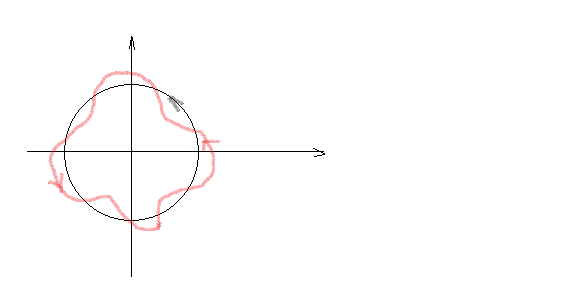
\includegraphics[width=8cm, height=4cm]{ch10/1}
 	\end{center} 
 	
 	Из непрерывной зависимости решения дифференциального уравнения от правой части(неоднородное уравнение) на данном промежутке времени(на периоде) следует, что траектория возмущённой системы не может далеко уйти от траектории невозмущённой системы.\\
 	
 	Рассмотрим гамильтониан(описывающий энергию системы) для системы (2):
 	\[
 	H=\dfrac{1}{2}(x_1^2 + x_2^2).
 	\]
 	\(\dot H = 0\), т.к. это П.И.\\
 	Период обозначим за  \(T_{\epsilon}\).\\
 	
 	
 	Рассмотрим (2):
 	\[
 	\dot H_{\epsilon} = x_1 \dot x_1 + x_2 \dot x_2 = \epsilon(x_1 f_1(x_1, x_2) + x_2 f(x_1, x_2)) \neq 0  \quad \Rightarrow
 	\]
 	\(
 	\Delta \dot H_{\epsilon}  = \{\Delta \dot H_{\epsilon}\) ---  изменение энергии за один оборот\(\}= \)
 	\[
 	=\epsilon \int \limits_0^{T_{\epsilon}} x_1 f_1(x_1, x_2) + x_2 f_2(x_1, x_2) \, dt = \epsilon \int \limits_0^{T} x_1 f_1(x_1, x_2) + x_2 f_2(x_1, x_2) \, dt  + O(\epsilon^2) 
 	\]
 	\[
 	T_{\epsilon}-T \sim\epsilon \quad \Rightarrow \quad \int \limits_0^{T_{\epsilon}} =  \int \limits_0^{T} + \epsilon
 	\]
 	\[
 	\Rightarrow \Delta \dot H_{\epsilon} = \epsilon \int_0^T F(R, t) \, dt + O(\epsilon^2)=\epsilon \Phi(R) + O(\epsilon^2),
 	\]
 	где \(F(R, t) = x_1^H f_1(x_1^H, x_2^H) + x_2^H f_2(x_1^H, x_2^H)\), \( \quad f_1, \, f_2\) --- гладкие.\\
 	
 	\begin{center}
 		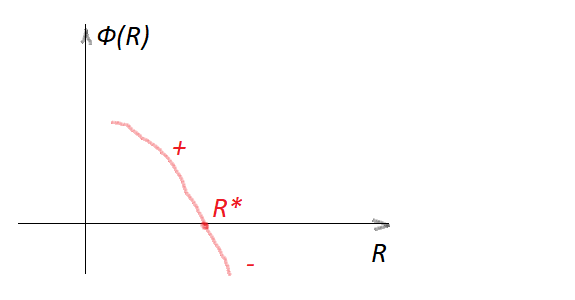
\includegraphics[width=8cm, height=4cm]{ch10/2}
 		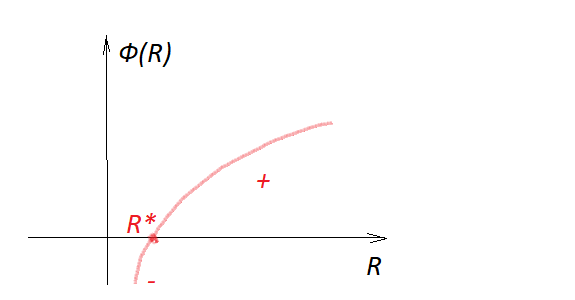
\includegraphics[width=8cm, height=4cm]{ch10/3}
 		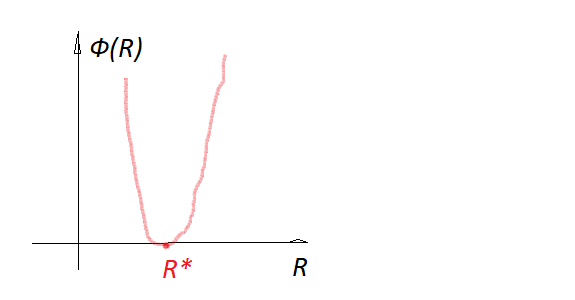
\includegraphics[width=8cm, height=4cm]{ch10/4}
 	\end{center}
 	\begin{center}
 		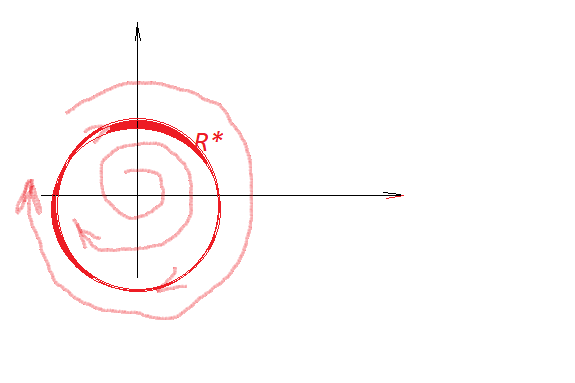
\includegraphics[width=9cm, height=6cm]{ch10/5}
 	\end{center}
 	Применим эту теорию к уравнению Ван-дер-Поля.\\
 	\[
 	\begin{cases}
 	\dot x_1 = x_2 - \left( \dfrac{x_1^3}{3} - x_1\right) \epsilon, \\
 	\dot x_2 = -x_1,\\
 	\end{cases}
 	f_1 = -\left( \dfrac{x_1^3}{3} - x_1\right), \quad f_2 = 0.
 	\]
 	Так как \(T_0 = 2\pi\), то:
 	\[
 	\Delta \dot H_{\epsilon} = \epsilon \int \limits_0^{2\pi} \left(x_1- \dfrac{x_1^3}{3}\right)x_1 \, dt +O(\epsilon^2) = \{  x_1 = R \cos t\} = \epsilon (I_1-I_2);
 	\]
 	\[
 	I_1 = \int \limits_0^{2\pi}  R^2 \cos^2 t dt = R^2\int \limits_0^{2\pi} \dfrac{1+\cos 2t}{2} \, dt = R^2 \pi,
 	\]
 	\[
 	I_2 = \int \limits_0^{2\pi}  \dfrac{R^4}{3} \cos^4 t \,dt = \dfrac{R^4}{6} \int \limits_0^{2\pi} (1 + \cos 2t)^2 ,\ dt = \dfrac{R^4}{12} \int \limits_0^{2\pi}(1  + \cos 2t + \cos ^2 2t) \, dt=
 	\]
 	\[
 	=\dfrac{R^4\pi}{6} + \dfrac{R^4}{24} \int \limits_0^{2\pi}(1 + \cos 4t) \,dt = \dfrac{R^4\pi}{12}(2\pi + \dfrac{1}{2} 2\pi) = \dfrac{R^4 \pi}{4}.
 	\]
 	
 	\[
 	\Rightarrow \quad \Phi(R) = \pi R^2\left(1-\dfrac{R^2}{4} \right)
 	\]
 	\(\Rightarrow\) предельный цикл существует с \(R_{\epsilon} = 2\). 
 	\begin{center}
 		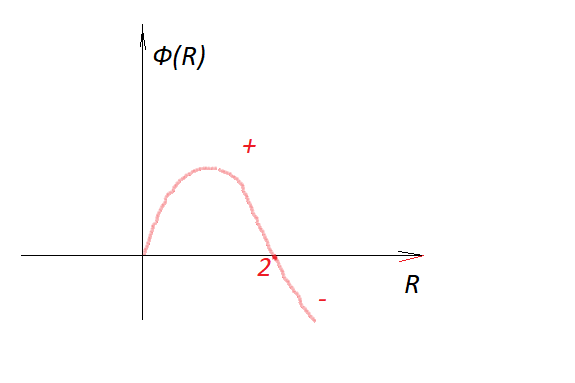
\includegraphics[width=10cm, height=7cm]{ch10/6}
 	\end{center}
 	
 	\clearpage
 	\[
 	\ddot x + g(x) \dot x + h(x) = 0
 	\]
 	\[
 	G(x) = \int \limits_0^x g(x) \, dx,
 	\]
 	\( G(x)\)  --- нечётная, \(G(x) \rightarrow +\infty\) при \(x  \rightarrow +\infty\).\\
 	\(h(x) > 0, \quad x > 0, \quad h(x)\) --- нечётная.\\
 	\[
 	\dfrac{d}{dt}(\dot x + G(x)) +h(x) =0.
 	\]
 	Пусть \(x_1 = x, \quad x_2 = \dot x + G(x)\), тогда имеет место система(3):
 	\[
 	\begin{cases}
 	\dfrac{x_1}{dt} = x_2 - G(x_1), \\
 	\dfrac{x_2}{dt} = -h(x_1),\\
 	\end{cases}
 	h(x_1) = x_1.
 	\]
 	Справедлива следующая теорема:
 	\begin{theorem}
 		\(G'(0) < 0, \quad |G'(0)|<2, \quad G\) --- гладкая. Тогда фазовый портрет системы (3) имееет предельный цикл, рождающийся из неустойчивого фокуса.
 	\end{theorem}
 	\begin{proof}
 		Положение равновесия \(x_1 = x_2 = 0\), \(h=x_1\).\\
 		\[
 		J = \begin{pmatrix}
 		-\dfrac{\partial G}{\partial x_1}	 &  1\\
 		-\dfrac{\partial h}{\partial x_1} & 0 \\
 		\end{pmatrix}
 		\]
 		\(
 		\lambda_{1,2} = \dfrac{-G'(0) +- \sqrt{(G'(0))^2-4}}{2}, \quad \Rightarrow \quad (0,0)\) --- неустойчивый фокус.\\
 		Если \((x_1, x_2) \rightarrow (-x_1, -x_2)\), то система не изменится.
 		\[
 		\dot x_1 = 0 \quad \Rightarrow \quad x_2 = G(x_1),
 		\]
 		\[
 		\dot x_2 = 0  \quad \Rightarrow \quad -x_1 = 0.
 		\]
 		\[
 		\begin{cases}
 		-\dfrac{x_1}{dt} = -x_2 + G(x_1), \\
 		-\dfrac{x_2}{dt} = h(x_1),\\
 		\end{cases}
 		\Leftrightarrow \quad  (3)
 		\]
 		Следовательно, можно рассматривать фазовый портрет в полуплоскости:
 		\begin{center}
 			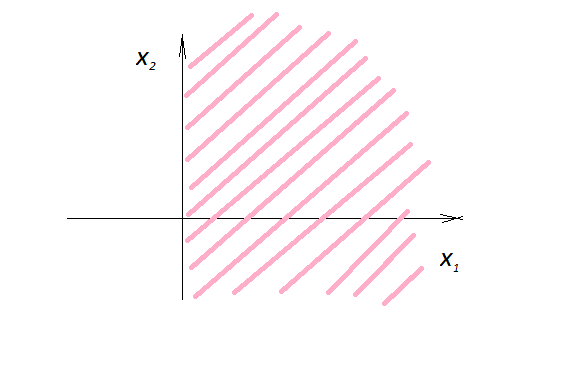
\includegraphics[width=8cm, height=4cm]{ch10/7}
 		\end{center}
 		\[
 		R = \dfrac{1}{2}(x_1^2 + x_2^2)  =R(t)
 		\]
 		\[
 		\dot R = x_1 \dot x_1 +x_2 \dot x_2 = x_1(x_2 - G(x_1))-x_2 x_1 = -x_1G(x_1)
 		\]\begin{center}
 			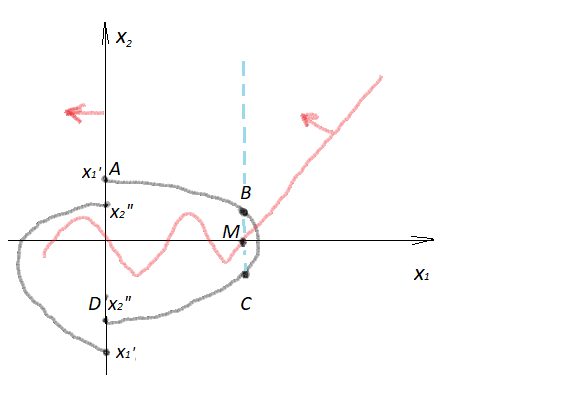
\includegraphics[width=10cm, height=7cm]{ch10/8}
 		\end{center}
 		\[
 		x_2 = l(x_1),
 		\]
 		\[
 		dt = \dfrac{dx_1}{x_2(x_1)} - G(x_1).
 		\]
 		\[
 		I_1 = \int\limits_A^B dR = \int \limits_{t_A}^{t_B} -x_1 G(x_1) dt = \{\overarc{AB}\} = -\int \limits_0^{M}\dfrac{x_1G(x_1)}{x_2 - G(x_1)}dx_1
 		\]
 		\[
 		I_2 = \int \limits_B^C dR = -\int \limits_{t_B}^{t_C} x_1 G(x_1) dt = \int \limits_B^C G(x_1(x_2)) dx_2= -\int\limits_C^B G(x_1(x_2))dx_2.
 		\]
 		\(
 		J_1\) --- ограниченная величина, \(J_2\) зависит от точки \(x_2'\).\\
 		
 		Замечание: \(J_{CD}\) тоже огранич., как и \(J_{AB}\).\\
 		Существует \(x_2'\) такое, что \(J_{CD} + J_{AB} + J_{BC}<0\).\\
 		По теореме Бендиксона-Пуанкаре имеется инвариантная область, нет особых точек, следовательно, предельный цикл устойчивый.
 	\end{proof}